\documentclass[aspectratio=169]{beamer}

\usepackage[utf8]{inputenc}
\usepackage{graphicx}
\usepackage{tikz}
\usetikzlibrary{positioning, arrows.meta}
\usepackage{pifont}

\usefonttheme{professionalfonts}

% Theme
\usetheme{Madrid}
\definecolor{ucdgreen}{RGB}{0, 102, 51}
\definecolor{gapred}{RGB}{180, 50, 50}
\definecolor{stepfill}{RGB}{230, 243, 235}
\usecolortheme[named=ucdgreen]{structure}
\setbeamertemplate{navigation symbols}{}

\title[Research Studies Panel]{Research Studies Panel}
\author[Lainey Ward]{Lainey Ward}
\institute[]{Decarb-AI Centre, School of Civil Engineering\\
Primary supervisor: Dr Fiachra O'Loughlin \\ Co-supervisor: Dr Conor Sweeney}
\date{}

\begin{document}

% --------------------------------------------------
% SLIDE 3: The system comparison — what I'm doing
% --------------------------------------------------
% PURPOSE: Show experimental setup concisely, then let
%          two plots carry the evidence. Script does the
%          explaining; slide shows the data.
% --------------------------------------------------
\begin{frame}{System Comparison: EEFH vs SEAS5}

    \begin{columns}[c, totalwidth=\textwidth]

        \begin{column}{0.38\textwidth}
            \centering
            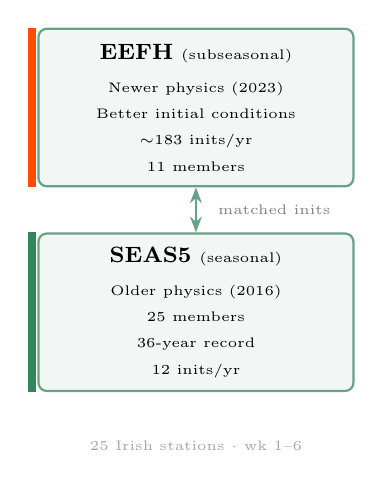
\begin{tikzpicture}[
                sysbox/.style={draw=ucdgreen!60, thick, rounded corners=3pt,
                    minimum width=4.0cm, minimum height=2.0cm,
                    fill=ucdgreen!5, align=center, font=\footnotesize},
                lbl/.style={font=\tiny, text=gray!70},
                tradeoff/.style={font=\tiny, text=gray!60, align=center}
            ]

            % EEFH
            \node[sysbox] (eefh) at (0, 2.2)
                {\textbf{EEFH} {\tiny(subseasonal)}\\[0.3em]
                 {\tiny Newer physics (2023)}\\
                 {\tiny Better initial conditions}\\
                 {\tiny $\sim$183 inits/yr}\\
                 {\tiny 11 members}};
            \fill[orange!60!red] ([xshift=-0.5pt]eefh.north west)
                rectangle ([xshift=-3.5pt]eefh.south west);

            % SEAS5
            \node[sysbox] (seas) at (0, -0.4)
                {\textbf{SEAS5} {\tiny(seasonal)}\\[0.3em]
                 {\tiny Older physics (2016)}\\
                 {\tiny 25 members}\\
                 {\tiny 36-year record}\\
                 {\tiny 12 inits/yr}};
            \fill[ucdgreen!80] ([xshift=-0.5pt]seas.north west)
                rectangle ([xshift=-3.5pt]seas.south west);

            % Comparison annotation
            \draw[{Stealth[length=2mm]}-{Stealth[length=2mm]},
                  thick, ucdgreen!60]
                (eefh.south) -- (seas.north)
                node[midway, right=0.15cm, font=\tiny, text=gray]
                {matched inits};

            % Verification target
            \node[lbl, below=0.5cm of seas]
                {25 Irish stations $\cdot$ wk 1--6};

            \end{tikzpicture}
        \end{column}

        \begin{column}{0.60\textwidth}
            % === PLOT PLACEHOLDERS ===
            % Replace these with \includegraphics when figures are ready

            \onslide<2->{
            
\begin{tikzpicture}
                \node[draw=gray!30, dashed, rounded corners,
                      minimum width=7.5cm, minimum height=3.0cm,
                      fill=gray!3, font=\footnotesize\color{gray!50}]
                    {Plot 1};
            \end{tikzpicture}
            }

            \vspace{0.3em}

            \onslide<3->{
            
\begin{tikzpicture}
                \node[draw=gray!30, dashed, rounded corners,
                      minimum width=7.5cm, minimum height=3.0cm,
                      fill=gray!3, font=\footnotesize\color{gray!50}]
                    {Plot 2};
            \end{tikzpicture}
            }
        \end{column}

    \end{columns}

\end{frame}

\end{document}